\documentclass[conference]{IEEEtran}

% Standard IEEE packages
\usepackage{cite}
\usepackage{amsmath,amssymb,amsfonts}
\usepackage{graphicx}
\usepackage{textcomp}
\usepackage{xcolor}
\usepackage{hyperref}
\usepackage{float}
\usepackage{booktabs}  % Professional tables

% Custom style file
\usepackage{ProjectReport}

\begin{document}

\title{MLB Game Simulation Dashboard:\\A Lambda Architecture Approach}

\author{
  \IEEEauthorblockN{Aadarsha Gopala Reddy}
  \IEEEauthorblockA{Department of Computer Science \& Engineering\\
    Washington University in St.\ Louis\\
    St.\ Louis, MO, USA\\
    a.gopalareddy@wustl.edu}
  \and
  \IEEEauthorblockN{Eddy Sul}
  \IEEEauthorblockA{Department of Computer Science \& Engineering\\
    Washington University in St.\ Louis\\
    St.\ Louis, MO, USA\\
    eddysul@wustl.edu}
}

\maketitle

% ============================================================
\begin{abstract}
  We present an interactive analytics dashboard for Major League Baseball (MLB) using \term{lambda architecture}. Our system combines batch processing of historical \statcast{} data (2015--2025) with a streaming layer that enables realistic game simulation. The pipeline uses \kafka{} for stream processing, \spark{} for micro-batch operations, \snowflake{} for data warehousing, and \airflow{} for orchestration. Users can explore historical games, analyze team matchups, and simulate past games pitch-by-pitch with configurable playback speeds.
\end{abstract}

\begin{IEEEkeywords}
  baseball analytics, real-time streaming, lambda architecture, Apache Kafka, Spark Streaming, data visualization
\end{IEEEkeywords}

% ============================================================
\section{Introduction}

The introduction of Statcast in 2015 transformed statistical analysis across Major League Baseball (MLB). Before 2015, MLB analytics primarily relied on static, historical box-score data. Statcast facilitated a shift from 2D to 3D analytics, capturing granular pitching metrics such as velocity and spin rate, as well as exit velocity and launch angle for every batted ball. This abundance of new data has empowered teams to develop novel strategies for a competitive edge.

Most of this data is accessible via Baseball Savant, which provides advanced analytics and visualizations. Additionally, MLB Gameday allows viewers to watch live game simulations. However, existing tools often segregate these functions: MLB Gameday focuses on real-time streaming without deep historical context, while other platforms lack interactive simulation capabilities. To bridge this gap, we developed an interactive dashboard that integrates game simulation with statistical analysis backed by comprehensive historical data. Specifically, our system augments the simulation with aggregational statistics—such as a hitter's performance against specific pitch types—and enables users to replay past games.

% ============================================================
\section{System Architecture}

Our system follows lambda architecture (Fig.~\ref{fig:pipeline}), combining two processing layers:

\begin{figure}[H]
  \centering
  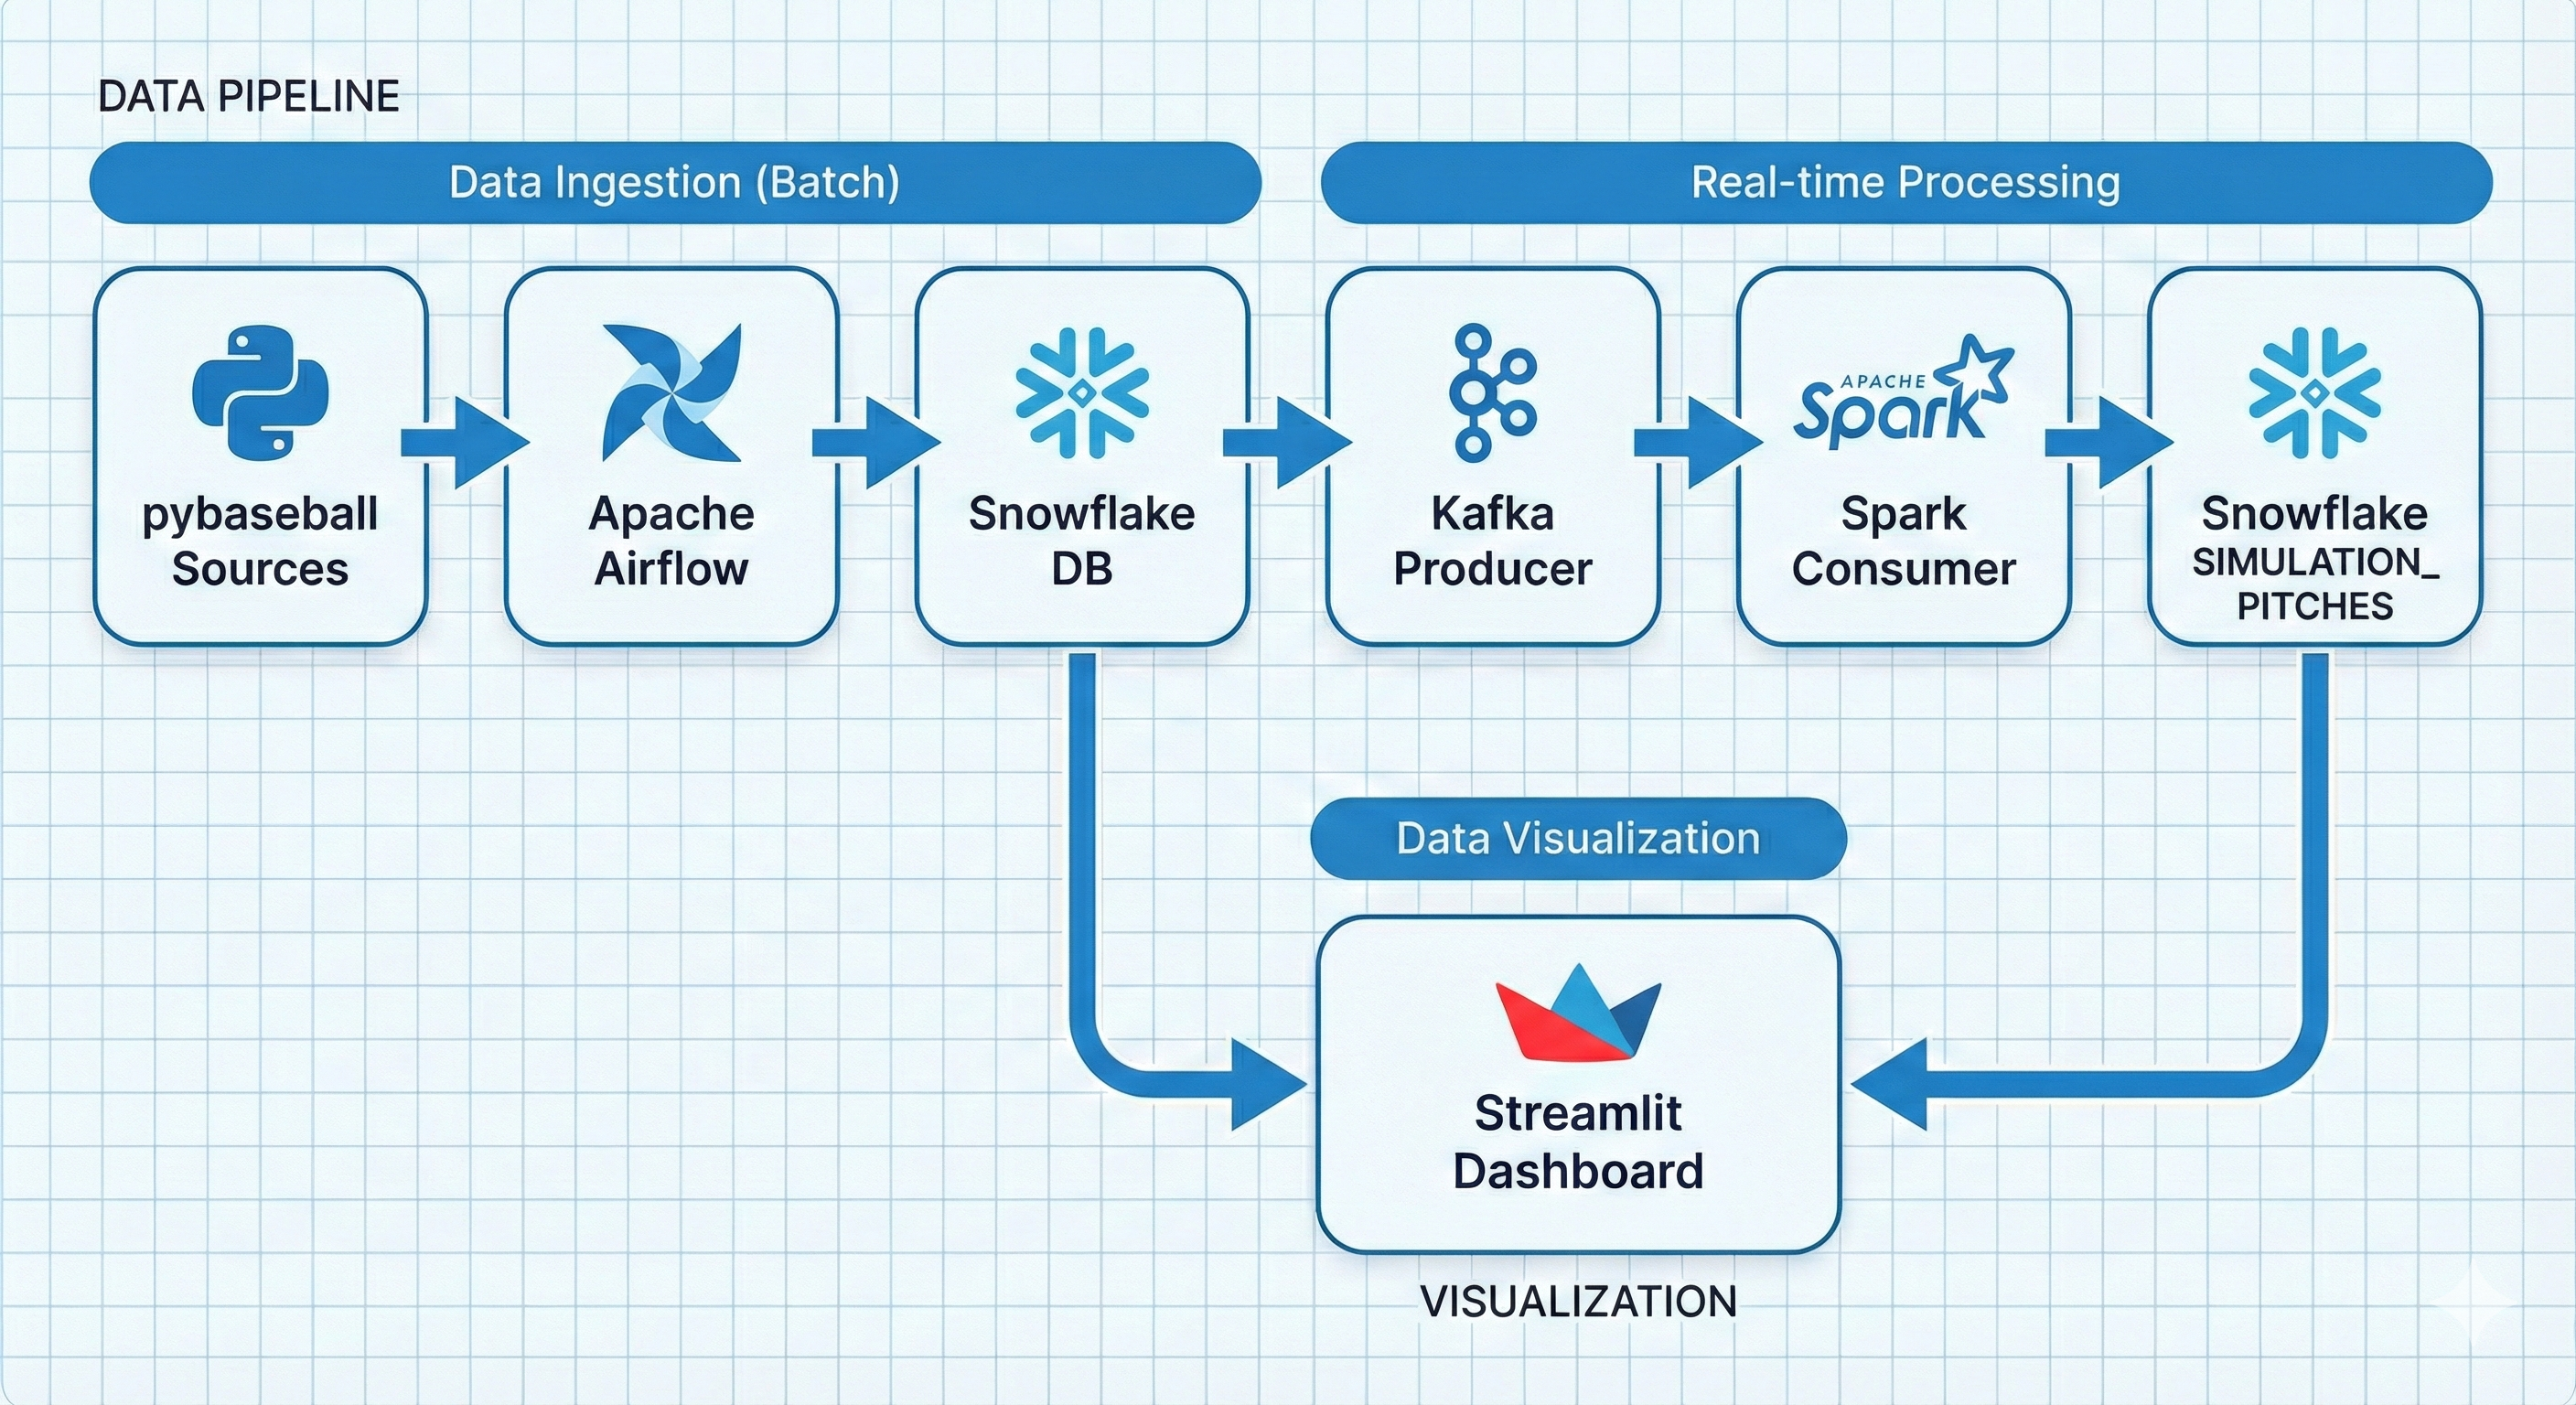
\includegraphics[width=0.48\textwidth]{Data Pipeline.png}
  \caption{Lambda architecture overview with batch and streaming layers.}
  \label{fig:pipeline}
\end{figure}

\begin{itemize}
  \item \layer{Batch Layer:} Daily ingestion of historical data via \airflow{} DAGs, stored in \snowflake{} using a star schema.
  \item \layer{Streaming Layer:} \kafka{} and \spark{} Streaming process pitch events for game simulation updates.
\end{itemize}

% ============================================================
\section{Data Pipeline}

\subsection{Ingestion and Transformation}

We use \texttt{pybaseball}, a Python wrapper for the MLB API, to fetch pitch-by-pitch logs. Each pitch contains over 118 fields; we filter these to retain only metrics relevant to our analysis. Although \texttt{pybaseball} does not support real-time streaming, it offers the most comprehensive daily-updated dataset dating back to 2015. We evaluated other APIs for real-time capabilities but found them either lacking in comprehensive metrics, incompatible with our stack, or prohibitively difficult to access.

The processing workflow:
\begin{enumerate}
  \item Fetch daily data via \texttt{pybaseball}
  \item Transform: remove deprecated fields, nulls, and out-of-scope metrics
  \item Stage as Parquet files in \snowflake{}
  \item Load into star schema tables
  \item Execute data quality checks
\end{enumerate}

\subsection{Database Schema}

We employ a \term{star schema} optimized for OLAP queries:

\begin{itemize}
  \item \textbf{Fact table:} \dbtable{fact\_pitches} --- one row per pitch
  \item \textbf{Dimensions:} \dbtable{player}, \dbtable{team}, \dbtable{pitch\_type}, \dbtable{game}
\end{itemize}

\subsection{Orchestration}

\airflow{} DAGs manage the pipeline (Fig.~\ref{fig:batch1}--\ref{fig:batch2}):

\begin{figure}[H]
  \centering
  \includegraphics[width=0.48\textwidth]{Batch Processing.png}
  \caption{Daily ingestion DAG.}
  \label{fig:batch1}
\end{figure}

\begin{figure}[H]
  \centering
  \includegraphics[width=0.48\textwidth]{Batch Processing 2.png}
  \caption{Historical backfill DAG (runs every 3 minutes).}
  \label{fig:batch2}
\end{figure}

% ============================================================
\section{Streaming Layer}

The streaming pipeline consists of three components:

\begin{enumerate}
  \item \textbf{\fastapi{} Producer:} Queries \snowflake{} and publishes pitch events to \kafka{}
  \item \textbf{\kafka{} Broker:} Buffers events (Docker container with Zookeeper)
  \item \textbf{\spark{} Consumer:} Processes micro-batches and writes to \dbtable{Live\_Pitches}
\end{enumerate}

\textbf{Decoupling Strategy:} Directly consuming the high-throughput stream in \streamlit{} can lead to dropped frames due to the framework's refresh latency. To mitigate this, we decoupled the visualization from the ingestion pipeline. The dashboard independently polls the \dbtable{Live\_Pitches} table, ensuring complete pitch sequence accuracy, albeit with marginally increased latency.

\begin{tradeoff}
  Data accuracy over minimal latency. Missing pitches would confuse viewers; slight delay is acceptable.
\end{tradeoff}

% ============================================================
\section{Dashboard Features}

\subsection{Game Explorer}
Select historical games and analyze pitcher statistics: velocity per pitch type, spin rate, and strikeout percentage. Includes strike zone visualization and velocity progression tracking.

\begin{figure}[H]
  \centering
  \includegraphics[width=0.48\textwidth]{Pitcher Performance.png}
  \caption{Pitcher repertoire breakdown and key statistics.}
  \label{fig:pitcher}
\end{figure}

\begin{figure}[H]
  \centering
  \includegraphics[width=0.48\textwidth]{Velocity.png}
  \caption{Pitch velocity progression throughout the game.}
  \label{fig:velocity}
\end{figure}

\subsection{Team Matchups}
Compare head-to-head statistics between teams across a season (Fig.~\ref{fig:matchup}).

\begin{figure}[H]
  \centering
  \includegraphics[width=0.48\textwidth]{Game Matchup.png}
  \caption{Team matchup: pitcher vs.\ batter statistics.}
  \label{fig:matchup}
\end{figure}

\subsection{Game Simulation}
Watch historical games unfold pitch-by-pitch with playback controls (0.5--5 pitches/second). This feature allows users to replay any past game. Notably, while the replay speed is not a 1:1 real-time mirror, it provides a highly customizable visualization tool for tactical analysis.

\begin{figure}[H]
  \centering
  \includegraphics[width=0.48\textwidth]{Game Simulation.jpg}
  \caption{Game simulation with game state and playback controls.}
  \label{fig:simulation}
\end{figure}

% ============================================================
\section{Challenges and Design Decisions}

\subsection{Schema Design}
With 110+ fields per pitch, we invested significant effort selecting relevant columns and designing intuitive dimension tables.

\subsection{Views vs.\ Materialized Tables}
We chose \snowflake{} views for dashboard aggregations:

\begin{table}[H]
  \centering
  \caption{Views vs.\ Materialized Tables Trade-offs}
  \begin{tabular}{@{}lcc@{}}
    \toprule
    \textbf{Factor}     & \textbf{Views} & \textbf{Materialized} \\
    \midrule
    Auto-sync with data & \checkmark     & Requires refresh      \\
    Query performance   & Slower         & Faster                \\
    Staleness risk      & None           & Possible              \\
    Our choice          & \checkmark     & ---                   \\
    \bottomrule
  \end{tabular}
\end{table}

For our workload (frequent writes, user-triggered reads), views provided acceptable latency with guaranteed consistency.

\subsection{Dashboard Latency}
\streamlit{}, depending on the system it is running on, imposes $\sim$1 second minimum refresh. Our \kafka{} producer can emit faster, but the dashboard cannot display sub-second updates. WebSocket-based alternatives (Dash, React) could improve this.

\subsection{Historical Data Range}
We focused on 2020--present for two reasons:
\begin{enumerate}
  \item Data quality improved post-2019 with upgraded tracking hardware
  \item Smaller backfill enabled faster development iteration
\end{enumerate}
The pipeline supports 2015+ data with minimal modification.

\subsection{Infrastructure Issues}
We encountered significant environment-specific dependency conflicts when migrating \airflow{} from a local development environment to the LinuxLab production server.

% ============================================================
\section{Future Work}

\subsection{True Real-Time Integration}
Current limitation: \texttt{pybaseball} provides data with $\sim$1-day delay.

\textbf{Required changes for live-season support:}
\begin{enumerate}
  \item WebSocket connection to MLB Gameday API
  \item \kafka{} producer emitting events as they arrive
  \item Reconciliation logic: merge real-time events with next-day \statcast{} data
\end{enumerate}

Our lambda architecture already supports this---streaming layer handles live events; batch layer provides quality-assured corrections.

\subsection{Data Corrections}
MLB issues scoring changes and data corrections. Potential solutions:
\begin{itemize}
  \item Change Data Capture (CDC) to detect source modifications
  \item Targeted updates to affected records
  \item Handle suspended games spanning multiple dates
\end{itemize}

\subsection{Performance Optimizations}
\begin{itemize}
  \item \textbf{\redis{} caching:} Lower latency for live updates
  \item \textbf{\flink{} streaming:} Event-by-event processing (vs.\ \spark{} micro-batches)
  \item \textbf{Materialized views:} For high-concurrency scenarios
\end{itemize}

\subsection{Additional Data Sources}

\begin{table}[H]
  \centering
  \caption{Potential Data Sources and Applications}
  \begin{tabular}{@{}p{2.2cm}p{2.5cm}p{2.8cm}@{}}
    \toprule
    \textbf{Data Type} & \textbf{Source/Library}             & \textbf{Application}                                                                 \\
    \midrule
    Weather            & OpenWeatherMap API, Visual Crossing & Correlate temperature, humidity, and wind with pitch movement and home run distances \\
    \addlinespace
    Stadium Info       & MLB Park Factors, Chadwick Bureau   & Normalize statistics across venues; account for altitude effects (e.g., Coors Field) \\
    \addlinespace
    Historical Stats   & Baseball Reference, Lahman Database & All-time head-to-head matchups; career splits analysis                               \\
    \addlinespace
    Player Tracking    & MLB Film Room API                   & Defensive positioning; sprint speed correlations                                     \\
    \bottomrule
  \end{tabular}
\end{table}

These integrations would enable advanced analytics such as weather-adjusted ERA, venue-normalized exit velocity, and predictive matchup modeling based on historical tendencies.

\subsection{Planned Features}
Batter splits against specific pitch types:
\begin{center}
  \textit{Ohtani vs.\ Righty Sliders: .333 Average}
\end{center}

% ============================================================
\section{Demonstration}

\begin{itemize}
  \item \textbf{Video demo:} \url{https://www.youtube.com/watch?v=z01fHvzd-8w}
  \item \textbf{Source code:} \url{https://github.com/agopalareddy/CSE-5114-Project}
\end{itemize}

% ============================================================
\section{Conclusion}
We presented an MLB game simulation dashboard combining batch and streaming processing via lambda architecture. The system demonstrates effective integration of \kafka{}, \spark{}, \snowflake{}, and \airflow{} for interactive baseball analytics, enabling users to replay historical games and explore detailed statistics. Future work includes true real-time integration during live seasons.

% ============================================================
\begin{thebibliography}{00}
  \bibitem{b1} MLB Advanced Media, ``Statcast,'' \url{https://www.mlb.com/glossary/statcast}.
  \bibitem{b2} Baseball Savant, ``Statcast Search,'' \url{https://baseballsavant.mlb.com/statcast_search}.
  \bibitem{b3} pybaseball, ``Python package for baseball data,'' \url{https://github.com/jldbc/pybaseball}.
  \bibitem{b4} Apache Kafka, \url{https://kafka.apache.org/}.
  \bibitem{b5} Apache Spark, \url{https://spark.apache.org/}.
  \bibitem{b6} Snowflake Inc., \url{https://www.snowflake.com/}.
\end{thebibliography}

\end{document}
